%%%%%%%%%%%%%%%%%%%%%%%%%%%%%%%%%%%%%%%%%%%%%%%%%%%%%%%%%%%%%%%
%
% Welcome to Overleaf --- just edit your LaTeX on the left,
% and we'll compile it for you on the right. If you give
% someone the link to this page, they can edit at the same
% time. See the help menu above for more info. Enjoy!
%
%%%%%%%%%%%%%%%%%%%%%%%%%%%%%%%%%%%%%%%%%%%%%%%%%%%%%%%%%%%%%%%
\documentclass[12pt]{article}
\usepackage[english]{babel}
\usepackage[utf8x]{inputenc}
\usepackage{amsmath}
\usepackage{tikz}
\usetikzlibrary{arrows,automata}
\begin{document}
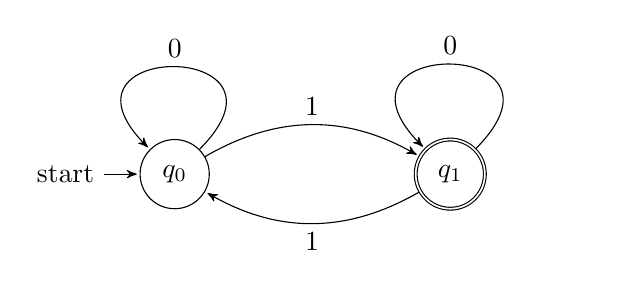
\begin{tikzpicture}[->,>=stealth',shorten >=1pt,auto,node distance=3.5cm,
        scale = 1,transform shape]

  \node[state,initial] (q_0) {$q_0$};
  \node[state,accepting] (q_1) [right of=q_0] {$q_1$};

  \path (q_0) edge[loop, looseness=8]              node[label=above:{$0$}] {} (q_0)
        (q_0) edge[bend left]              node {$1$} (q_1)
        (q_1) edge[loop, looseness=8]              node[label=above:{$0$}] {}(q_1)
        (q_1) edge[bend left]              node {$1$} (q_0);

\end{tikzpicture}
\end{document}
%%%%%%%%%%%%%%%%%%%%%%%%%%%%%%%%%%%%%%%%%%%%%%%%%%%%%%%%%%%%%%%
%
% Welcome to Overleaf --- just edit your LaTeX on the left,
% and we'll compile it for you on the right. If you give
% someone the link to this page, they can edit at the same
% time. See the help menu above for more info. Enjoy!
%
%%%%%%%%%%%%%%%%%%%%%%%%%%%%%%%%%%%%%%%%%%%%%%%%%%%%%%%%%%%%%%%
\documentclass[12pt]{article}
\usepackage[english]{babel}
\usepackage[utf8x]{inputenc}
\usepackage{amsmath}
\usepackage{tikz}
\usetikzlibrary{arrows,automata}
\begin{document}
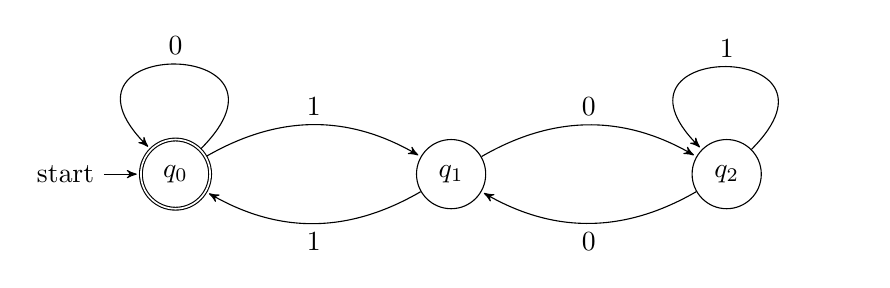
\begin{tikzpicture}[->,>=stealth',shorten >=1pt,auto,node distance=3.5cm,
        scale = 1,transform shape]

  \node[state,accepting,initial] (q_0) {$q_0$};
  \node[state] (q_1) [right of=q_0] {$q_1$};
  \node[state] (q_2) [right of=q_1] {$q_2$};

  \path (q_0) edge [loop, looseness=8]              node[label=above:{$0$}] {} (q_0)
        (q_0) edge [bend left]             node {$1$} (q_1)
        (q_1) edge [bend left]             node {$0$} (q_2)
        (q_1) edge [bend left]             node {$1$} (q_0)
        (q_2) edge [bend left]            node {$0$} (q_1)
        (q_2) edge [loop, looseness=8]             node [label=above:{$1$}]{} (q_2);

\end{tikzpicture}
\end{document}
%%%%%%%%%%%%%%%%%%%%%%%%%%%%%%%%%%%%%%%%%%%%%%%%%%%%%%%%%%%%%%%
%
% Welcome to Overleaf --- just edit your LaTeX on the left,
% and we'll compile it for you on the right. If you give
% someone the link to this page, they can edit at the same
% time. See the help menu above for more info. Enjoy!
%
%%%%%%%%%%%%%%%%%%%%%%%%%%%%%%%%%%%%%%%%%%%%%%%%%%%%%%%%%%%%%%%
\documentclass[12pt]{article}
\usepackage[english]{babel}
\usepackage[utf8x]{inputenc}
\usepackage{amsmath}
\usepackage{tikz}
\usetikzlibrary{arrows,automata}
\begin{document}
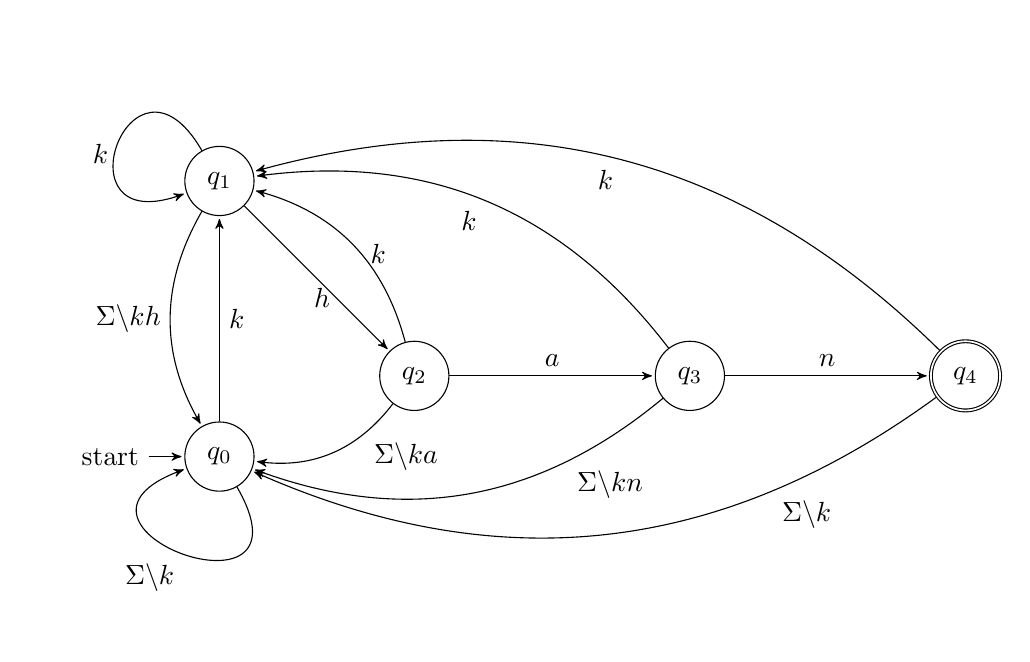
\begin{tikzpicture}[->,>=stealth',shorten >=1pt,auto,node distance=3.5cm,
        scale = 1,transform shape]

  \node[state,initial] (q_0) {$q_0$};
  \node[state] (q_1) [above of=q_0] {$q_1$};
  \node[state] (q_2) [below right of=q_1] {$q_2$};
  \node[state] (q_3) [right of=q_2] {$q_3$};
  \node[state,accepting] (q_4) [right of=q_3] {$q_4$};

  \path (q_0) edge [out=-60, in = 200, looseness=8]              node [label=below:{}] {$\Sigma\backslash k$} (q_0)
        (q_0) edge                                               node [label=right:{$k$}, pos=0.5]{} (q_1)
        (q_1) edge [out=120, in = 200, looseness=8]              node [label=left:{$k$}] {} (q_1)
        (q_1) edge                         node [label=below:{$h\ $}, pos=0.5] {} (q_2)
        (q_2) edge              node {$a$} (q_3)
        (q_3) edge              node {$n$} (q_4)
        (q_1) edge [bend right]             node [label=left:{$\Sigma\backslash kh$}, pos=0.5] {} (q_0)
        (q_2) edge [bend left]             node [label=above:, pos=0.25] {$\Sigma\backslash ka$} (q_0)
        (q_3) edge [bend left]             node [label=above:, pos=0.25] {$\Sigma\backslash kn$} (q_0)
        (q_4) edge [bend left]             node [label=above:, pos=0.25] {$\Sigma\backslash k$} (q_0)
        (q_2) edge [bend right]             node [label=right:{$\ k$}, pos=0.5] {} (q_1)
        (q_3) edge [bend right]             node [label=above:, pos=0.5] {$k$} (q_1)
        (q_4) edge [bend right]             node [label=above:, pos=0.5] {$k$} (q_1);

\end{tikzpicture}
\end{document}

\documentclass[12pt]{article}
\usepackage[english]{babel}
\usepackage[utf8x]{inputenc}
\usepackage{amsmath}
\usepackage{tikz}
\usetikzlibrary{arrows,automata}
\begin{document}
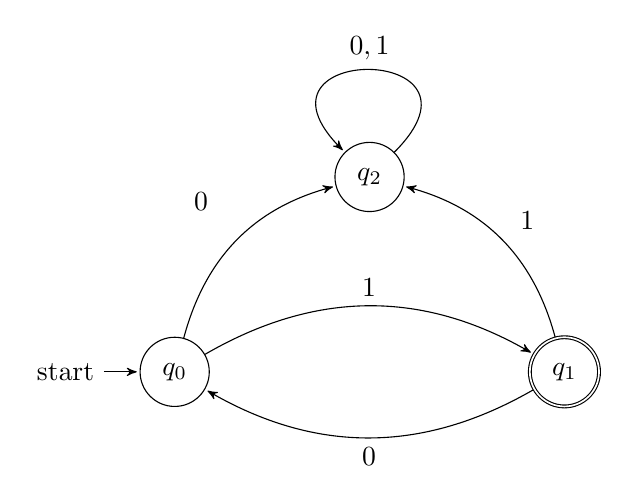
\begin{tikzpicture}[->,>=stealth',shorten >=1pt,auto,node distance=3.5cm,
        scale = 1,transform shape]

  \node[state,initial] (q_0) {$q_0$};
  \node[state] (q_2) [above right of=q_0] {$q_2$};
  \node[state, accepting] (q_1) [below right of=q_2] {$q_1$};
  

  \path (q_0) edge[bend left]              node[label=above left:{$0$}] {} (q_2)
        (q_0) edge[bend left]              node {$1$} (q_1)
        (q_1) edge[bend right]              node[label=above right:{$\ 1$}] {}(q_2)
        (q_1) edge[bend left]              node {$0$} (q_0)
        (q_2) edge [loop, looseness=8]    node[label=above:{$0, 1$}]{}(q_2);

\end{tikzpicture}
\end{document}